\documentclass[12pt, letterpaper]{article}

\usepackage[utf8]{inputenc}
\usepackage[ngerman]{babel}
\usepackage{graphicx}
\usepackage{fancyvrb}
\usepackage{float}
\usepackage{textcomp}
\usepackage{minted}
\usepackage{listings}

\graphicspath{ {./} }

\title{Prisoner's Dilemma}
\author{Matthias Grill}
\date{2019-03-05}

\begin{document}
	
\pagenumbering{gobble}
\maketitle
\newpage

\tableofcontents
\newpage

\pagenumbering{arabic}

\section{Lizenz}
\begin{Verbatim}
Boost Software License - Version 1.0 - August 17th, 2003

Permission is hereby granted, free of charge, to any person or
organization obtaining a copy of the software and accompanying
documentation covered by this license (the "Software") to use,
reproduce, display, distribute, execute, and transmit the
Software, and to prepare derivative works of the Software, and
to permit third-parties to whom the Software is furnished to do
so, all subject to the following:

The copyright notices in the Software and this entire statement,
including the above license grant, this restriction and the
following disclaimer, must be included in all copies of the
Software, in whole or in part, and all derivative works of the
Software, unless such copies or derivative works are solely in
the form of machine-executable object code generated by a source
language processor.

THE SOFTWARE IS PROVIDED "AS IS", WITHOUT WARRANTY OF ANY KIND,
EXPRESS OR IMPLIED, INCLUDING BUT NOT LIMITED TO THE WARRANTIES
OF MERCHANTABILITY, FITNESS FOR A PARTICULAR PURPOSE, TITLE AND
NON-INFRINGEMENT. IN NO EVENT SHALL THE COPYRIGHT HOLDERS OR
ANYONE DISTRIBUTING THE SOFTWARE BE LIABLE FOR ANY DAMAGES OR
OTHER LIABILITY, WHETHER IN CONTRACT, TORT OR OTHERWISE, ARISING
FROM, OUT OF OR IN CONNECTION WITH THE SOFTWARE OR THE USE OR
OTHER DEALINGS IN THE SOFTWARE.
\end{Verbatim}

\clearpage

\normalsize

\newpage

\section{Aufgabenstellung}
Aufgabe dieses Projekts ist es ein netzwerk-basiertes iteratives Prisoner's Dilemma mit zentralem Server zu implementieren. Wobei jeder Client die Möglichkeit hat seine eigene Strategie zu implementieren und anschließend diese gegen den anderen anzuwenden.

\subsection{Technologien}
Dieses Projekt wurde in C++17 mit der Hilfe von folgenden Technologien realisiert:
\begin{itemize}
	\item Meson
	\item Ninja
	\item Clipp
	\item Spdlog
	\item JSON
	\item Asio
	\item Google Protocol Buffers
\end{itemize}

\section{Spielerklärung}
Prisoner's Dilemma ist ein mathematisches Spiel aus der Spieltheorie. Es modelliert die Situation zweier Gefangener, die beschuldigt werden, gemeinsam ein Verbrechen begangen zu haben. Die beiden Gefangenen werden einzeln verhört und können nicht miteinander kommunizieren. Leugnen beide das Verbrechen, erhalten beide eine Strafe von zwei Jahren, da ihnen nur eine weniger streng bestrafte Tat nachgewiesen werden kann. Gestehen beide, erhalten beide dafür eine Strafe von vier Jahren, wegen ihres Geständnisses aber nicht die Höchststrafe. Gesteht jedoch nur einer der beiden Gefangenen, geht dieser als Kronzeuge mit nur einem Jahr Strafe aus, während der andere als überführter, aber nicht geständiger Täter die Höchststrafe von sechs Jahren bekommt.

\begin{table}[h]
	\centering
	\begin{tabular}{|c|c|c|}
		\hline
		& \textbf{\begin{tabular}[c]{@{}c@{}}Spieler B \\ kooperiert nicht\end{tabular}} & \textbf{\begin{tabular}[c]{@{}c@{}}Spieler B \\ kooperiert\end{tabular}} \\ \hline
		\textbf{\begin{tabular}[c]{@{}c@{}}Spieler A \\ kooperiert nicht\end{tabular}} & \begin{tabular}[c]{@{}c@{}}A: 2 Jahre\\ B: 2 Jahre\end{tabular}                & \begin{tabular}[c]{@{}c@{}}A: 6 Jahre\\ B: 1 Jahre\end{tabular}          \\ \hline
		\textbf{\begin{tabular}[c]{@{}c@{}}Spieler A\\  koopertiert\end{tabular}}      & \begin{tabular}[c]{@{}c@{}}A: 1 Jahre\\ B: 6 Jahre\end{tabular}                & \begin{tabular}[c]{@{}c@{}}A: 4 Jahre\\ B: 4 Jahre\end{tabular}          \\ \hline
	\end{tabular}
	\caption{Visualisierung der Spielregeln}
\end{table}

\section{Implementierung}

\subsection{Programmablauf}
\begin{enumerate}
	\item Server wird gestartet und wartet auf zwei Clients
	\item Client wird gestartet und schickt einen Join-Request an den Server
	\item Server schickt einen Confirm-Response an den Client zurück
	\item Wenn zwei Clients verbunden sind benachrichtigt der Server alle Clients über den Spielstart
	\item Ablauf für x Spielrunden:
	\begin{enumerate}
		\item Server wartet auf zwei Entscheidungen
		\item Clients schicken ihre Entscheidung
		\item Server schickt das Ergebnis an den jeweiligen Client zurück
	\end{enumerate}
	\item Server schickt das Endergebnis an alle Clients
	\item Server schließt die Verbindungen zu den Clients
	\item Clients schließen die Verbindung zum Server
	\item Clients beenden sich und Server startet neu
\end{enumerate}

\newpage

\subsection{Kommandozeilen Benutzerschnittstelle}
Die Kommandozeilen Benutzerschnittstelle wurde mit Hilfe von Clipp realisert. Folgende Schnittstellen werden zur Verfügung gestellt:

\paragraph{Prisoner's Dilemma Server}
\begin{Verbatim}[fontsize=\small]
SYNOPSIS
    ./server [-p <port>] [-r <rounds>] [-d] [-h]

OPTIONS
    -p, --port        Port to connect to
    -r, --rounds      Number of rounds you want to play
    -d, --debug       Debug mode
    -h, --help        Print this help message and exit
\end{Verbatim}

\paragraph{Prisoner's Dilemma Client}
\begin{Verbatim}
SYNOPSIS
    ./client [-st] [-s <ip>] [-p <port>] [-d] [-h]

OPTIONS
    -st, --strategy   Your own strategy will be used
    -s, --server      Ip adress of server
    -p, --port        Port to connect to
    -d, --debug       Debug mode
    -h, --help        Print this help message and exit
\end{Verbatim}

\paragraph{Beispiel-Aufrufe}
\begin{Verbatim}
./server
./server -p 8080
./server --rounds 5
./server -p 8080 --debug

./client
./client -p 8080
./client -d --strategy
./client -st --server "192.168.0.110" --debug
\end{Verbatim}

\subsection{Konfiguration}
Die Standardkonfiguration des Servers und Clients erfolgt mittels zwei verschiedener JSON-Dateien (Welche sich beide in /src/static befinden). Die Einstellungen welche hier getroffen werden, können jedoch durch die Kommandozeilen Benutzerschnittstelle überschrieben werden. 

\paragraph{Prisoner's Dilemma Server}

\begin{minted}[]{json}
{
    "port": 8081,
    "rounds": 3,
    "debug": false
}
\end{minted}

\begin{itemize}
	\item Port: Port auf dem der Server gestartet wird
	\item Rounds: Anzahl der Runden die gespielt werden
	\item Debug
	\begin{itemize}
		\item True: Debug-Nachrichten werden ausgegeben
		\item False: Debug-Nachrichten werden nicht ausgegeben
	\end{itemize}
\end{itemize}

\paragraph{Prisoner's Dilemma Client}

\begin{minted}[]{json}
{
    "playOnCommandLine": true,
    "serverIp": "localhost",
    "port": 8081,
    "debug": false
}
\end{minted}

\begin{itemize}
	\item PlayOnCommandLine
	\begin{itemize}
		\item True: Client kann die Entscheidungen auf der Kommandozeile treffen
		\item False: Es wird automatisch die eigens implementierte Strategie verwendet
	\end{itemize}
	\item ServerIp: IP-Adresse des Servers
	\item Port: Port des Servers
	\item Debug
	\begin{itemize}
		\item True: Debug-Nachrichten werden ausgegeben
		\item False: Debug-Nachrichten werden nicht ausgegeben
	\end{itemize}
\end{itemize}

\subsection{Google Protocol Buffers}
Zur Kommunikation zwischen Client und Server wird Asio zusammen mit Google Protocol Buffers verwendet. Die Protobuf Nachrichten werden serialisiert und anschließend über einen Asio Socket verschickt. Auf der anderen Seite des Sockets werden die Nachrichten empfangen und daraufhin wieder in eine Protobuf Nachricht geparsed.

\subsection{UML Klassendiagramm}

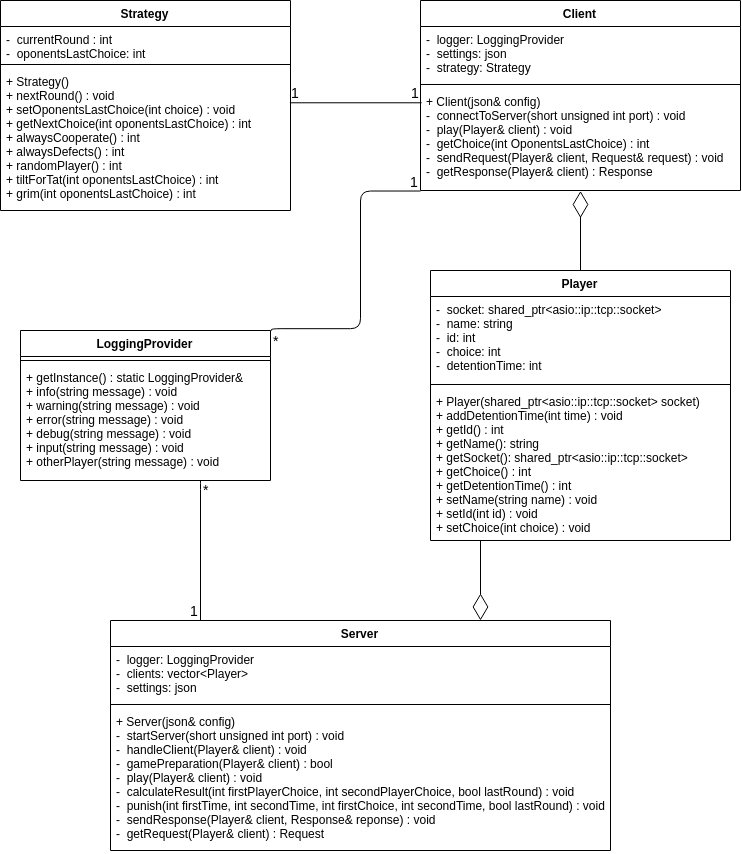
\includegraphics[width=\linewidth]{UML}

\section{Strategie}
Für den Client gibt es zwei verschiedene Möglichkeiten Prisoner's Dilemma zu spielen. Einerseits kann es auf der Kommandozeile spielen und anderseits gibt es auch eine zur Verfügung gestellte Schnittstelle, bei welcher es die Möglichkeit gibt, die eigene Strategie zu implementieren. Des Weiteren muss nicht jeder Client den gleichen Spielstil wählen, also ist es auch möglich, dass ein Spieler auf der Kommandozeile spielt und der andere verwendet seine eigene Strategie, welche er im vorhinein implementiert hat.

\subsection{Schnittstelle}
In der Strategy-Klasse gibt es für den Spieler die Möglichkeit seine eigene Strategie zu implementieren. Des Weiteren gibt es schon ein paar vordefinierte Strategien welche natürlich auch verwendet werden könnnen. Folgende Strategien sind bereits implementiert:

\begin{itemize}
	\item AlwaysCooperate: Kooperiert immer
	\item AlwaysDefects: Kooperiert nie
	\item RandomPlayer: Zufällige Entscheidung
	\item TiltForTat: Kooperiert beim ersten mal und ab dann entscheidet er sich immer für das selbe wie der andere Spieler in der Vorrunde
	\item Grim: Kooperiert so lange bis der andere Spiele kooperiert ab dann kooperiert er nicht mehr
\end{itemize}

\noindent
Will man einer dieser Strategien andwenden muss man sie in der getNextChoice() Methode aufrufe. Will der Spieler seine komplett eigene Strategie implementieren muss er diese ebenfalls in der getNextChoice() Methode implementieren. Folgende Variablen stehen ihm in dieser Funktion bereits zur Verfügung:

\begin{itemize}
	\item OpponentsLastChoice: Die Entscheidung des Gegner in der letzten Runde. In der ersten Runde beträgt der Wert -1, da es ja noch keine Entscheidung gab
	\item CurrentRound: Derzeitige Runde (Beginnend mit 1)
\end{itemize}

\end{document}